%%%%%%%%%%%%%%%%%%%%%%%%%%%%% Define Exam %%%%%%%%%%%%%%%%%%%%%%%%%%%%%%%%%%
\documentclass[addpoints]{exam}
%%%%%%%%%%%%%%%%%%%%%%%%%%%%%%%%%%%%%%%%%%%%%%%%%%%%%%%%%%%%%%%%%%%%%%%%%%%%%%%

%%%%%%%%%%%%%%%%%%%%%%%%%%%%% Using Packages %%%%%%%%%%%%%%%%%%%%%%%%%%%%%%%%%%
\usepackage{amsmath, amssymb, amsthm, amsfonts, geometry, venndiagram, tikz}
\usepackage{graphicx, xcolor, color, wrapfig, parskip, float, tabularx}
\usepackage[breaklinks]{hyperref}
\usepackage{colortbl, caption}
\usepackage{listings, mdframed, subfig, matlab-prettifier, hyperref}
\usepackage{lipsum, bookmark, booktabs, empheq, titlesec, verbatim, subfig, pdfpages, comment}

%%%%%%%%%%%%%%%%%%%%%%%%%%%%%%%%%%%%%%%%%%%%%%%%%%%%%%%%%%%%%%%%%%%%%%%%%%%%%%%
\definecolor{codebackground}{rgb}{0.95,0.95,0.95}
\definecolor{codegray}{rgb}{0.5,0.5,0.5}
\definecolor{codepurple}{rgb}{0.58,0,0.82}
\definecolor{codeblue}{rgb}{0.13,0.29,0.53}
\definecolor{ocre}{RGB}{243,102,25}
\definecolor{mygray}{RGB}{243,243,244}
\definecolor{deepGreen}{RGB}{26,111,0}
\definecolor{shallowGreen}{RGB}{235,255,255}
\definecolor{deepBlue}{RGB}{61,124,222}
\definecolor{shallowBlue}{RGB}{235,249,255}
\definecolor{softgray}{rgb}{0.95, 0.95, 0.95}
\definecolor{codegreen}{rgb}{0,0.6,0}
\definecolor{codegray}{rgb}{0.5,0.5,0.5}
\definecolor{codepurple}{rgb}{0.58,0,0.82}
\definecolor{backcolour}{rgb}{0.95,0.95,0.92}

%Code listing style named "mystyle"
\lstdefinestyle{mystyle}{
  backgroundcolor=\color{backcolour}, commentstyle=\color{codegreen},
  keywordstyle=\color{magenta},
  numberstyle=\tiny\color{codegray},
  stringstyle=\color{codepurple},
  basicstyle=\ttfamily\footnotesize,
  breakatwhitespace=false,         
  breaklines=true,                 
  captionpos=b,                    
  keepspaces=true,                 
  numbers=left,                    
  numbersep=5pt,                  
  showspaces=false,                
  showstringspaces=false,
  showtabs=false,                  
  tabsize=2
}

%"mystyle" code listing set
\lstset{style=mystyle}

\usetikzlibrary{arrows,shapes,positioning,shadows,trees, backgrounds}

\tikzstyle{arrow} = [->,>=stealth]
\tikzstyle{node} = [auto,font=\footnotesize,draw,circle]

%%%%%%%%%%%%%%%%%%%%%%%%%%%%% Header and Footer %%%%%%%%%%%%%%%%%%%%%%%%%%%%%%%%%%
\pagestyle{headandfoot}
\runningheadrule
\runningfootrule
\runningheader{Algorithms: Design and Analysis}{Weekly Challenge 06}{CS 412}
\runningfooter{}{Page \thepage\ of \numpages}{}
\firstpageheader{}{}{}
%%%%%%%%%%%%%%%%%%%%%%%%%%%%%%%%%%%%%%%%%%%%%%%%%%%%%%%%%%%%%%%%%%%%%%%%%%%%%%%

% Other Settings
% \boxedpoints
\printanswers
\qformat{}  %Comment this to number questions, uncomment this to not number questions

\newcommand\union\cup
\newcommand\inter\cap

%%%%%%%%%%%%%%%%%%%%%%%%%%%%%%% Title & Author %%%%%%%%%%%%%%%%%%%%%%%%%%%%%%%%

\title{Algorithms: Design and Analysis - CS 412 \vspace*{-4mm}}
\author{Weekly Challenge 06}
\date{\vspace*{-4mm} Ali Muhammad Asad - aa07190}

% \pgfplotsset{compat=1.18}

%%%%%%%%%%%%%%%%%%%%%%%%%%%%%%%%%%%%%%%%%%%%%%%%%%%%%%%%%%%%%%%%%%%%%%%%%%%%%%%

\begin{document}
\maketitle

% {\small \begin{center} \gradetable[h] \end{center}}
% \centerline{\rule{.7\textwidth}{1pt}}
\begin{questions}
  \question[1]
  Consider the graph, $\mathcal{G}$, below with 10 nodes and 13 edges.
  \begin{center}
    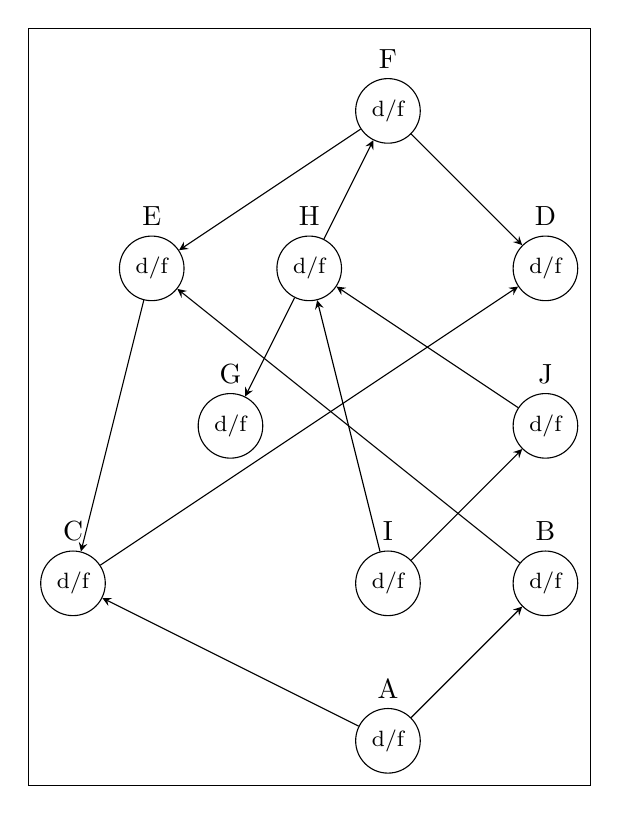
\begin{tikzpicture}[show background rectangle]
      \node[node] [anchor=north, label={A}] (a) at (5, 1) {d/f};
      \node[node] [anchor=north, label={B}] (b) at (7, 3) {d/f};
      \node[node] [anchor=north, label={C}] (c) at (1, 3) {d/f};
      \node[node] [anchor=north, label={D}] (d) at (7, 7) {d/f};
      \node[node] [anchor=north, label={E}] (e) at (2, 7) {d/f};
      \node[node] [anchor=north, label={F}] (f) at (5, 9) {d/f};
      \node[node] [anchor=north, label={G}] (g) at (3, 5) {d/f};
      \node[node] [anchor=north, label={H}] (h) at (4, 7) {d/f};
      \node[node] [anchor=north, label={I}] (i) at (5, 3) {d/f};
      \node[node] [anchor=north, label={J}] (j) at (7, 5) {d/f};

      \draw[arrow] (a) -- (c);
      \draw[arrow] (c) -- (d);
      \draw[arrow] (f) -- (d);
      \draw[arrow] (f) -- (e);
      \draw[arrow] (e) -- (c);
      \draw[arrow] (a) -- (b);
      \draw[arrow] (b) -- (e);
      \draw[arrow] (h) -- (f);
      \draw[arrow] (h) -- (g);
      \draw[arrow] (j) -- (h);
      \draw[arrow] (i) -- (h);
      \draw[arrow] (i) -- (j);
    \end{tikzpicture}
  \end{center}
  The procedure, $\text{DFS}(\mathcal{G})$, is executed on the graph such that ties are resolved in alphabetical order.
  \begin{parts}
    \part Redraw the graph below such that each node, $n$, contains $n.d/n.f$, where $n.d$ and $n.f$ are the node's discovery and finalization times respectively. Mention your starting nodes/nodes under the graph.
    \part Draw below the corresponding DFS-forest.
  \end{parts}

  \begin{solution}
    \begin{parts}
      \part The graph with discovery and finalization times is shown below.
      \begin{center}
        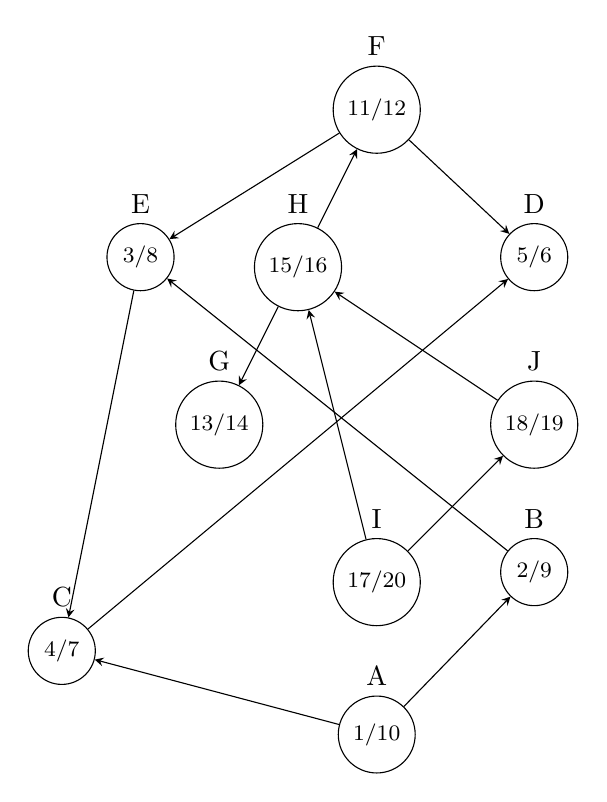
\begin{tikzpicture}
          \node[node] [anchor=north, label={A}] (a) at (5, 1) {1/10};
          \node[node] [anchor=north, label={B}] (b) at (7, 3) {2/9};
          \node[node] [anchor=north, label={C}] (c) at (1, 2) {4/7};
          \node[node] [anchor=north, label={D}] (d) at (7, 7) {5/6};
          \node[node] [anchor=north, label={E}] (e) at (2, 7) {3/8};
          \node[node] [anchor=north, label={F}] (f) at (5, 9) {11/12};
          \node[node] [anchor=north, label={G}] (g) at (3, 5) {13/14};
          \node[node] [anchor=north, label={H}] (h) at (4, 7) {15/16};
          \node[node] [anchor=north, label={I}] (i) at (5, 3) {17/20};
          \node[node] [anchor=north, label={J}] (j) at (7, 5) {18/19};

          \draw[arrow] (a) -- (c);
          \draw[arrow] (c) -- (d);
          \draw[arrow] (f) -- (d);
          \draw[arrow] (f) -- (e);
          \draw[arrow] (e) -- (c);
          \draw[arrow] (a) -- (b);
          \draw[arrow] (b) -- (e);
          \draw[arrow] (h) -- (f);
          \draw[arrow] (h) -- (g);
          \draw[arrow] (j) -- (h);
          \draw[arrow] (i) -- (h);
          \draw[arrow] (i) -- (j);
        \end{tikzpicture}
      \end{center}
      We are performing a DFS on $\mathcal{G}$, hence, we go as deep as we can before backtracking and moving onto any other node.

      Since the ties are resolved in alphabetical order, we start with the node $A$, since lexographically, it is the smallest node. From $A$, we move to $B$, then to $E$, then to $C$, then to $D$, marking the times as 1, 2, 3, 4, and 5 respectively. After $D$, we can't go any deeper, hence we mark its end time 6, and backtrack on our end times in the similar manner, marking times of 7, 8, 9, and 10 on nodes $C$, $E$, $B$, and $A$ respectively.

      Now there are no more nodes to go into, hence, we move onto the lexographically smallest node left from our set of nodes that the graph $\mathcal{G}$ is comprised of; $F$. We discover $F$, and mark its start time as 11, but we can't go deeper hence its end time becomes 12.

      We follow the same pattern again, with new starting nodes as $G$, $H$,   and $I$. We can move from $I$ to $J$, hence we don't include $J$ in the starting nodes. The set of starting nodes becomes $ \{ A, F, G, H, I \} $.

      \newpage
      \part The DFS-forest is shown below.

      \begin{center}
        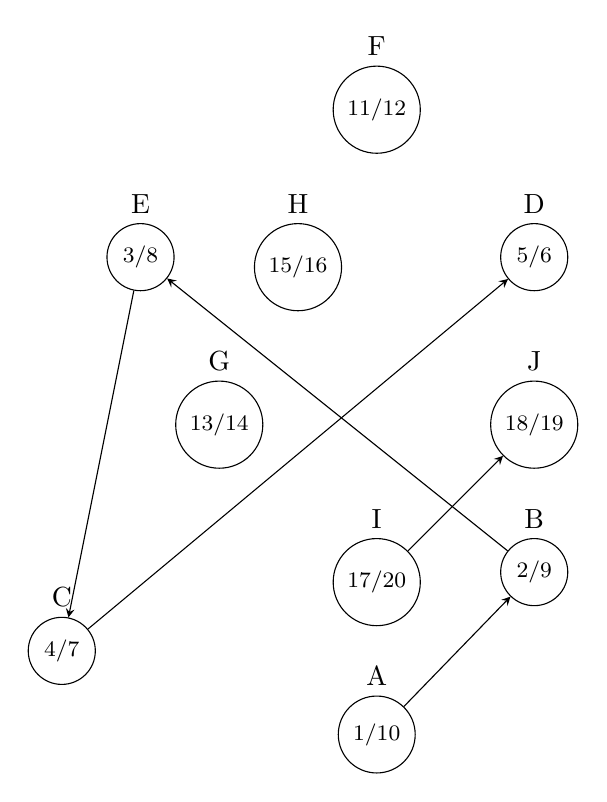
\begin{tikzpicture}
          \node[node] [anchor=north, label={A}] (a) at (5, 1) {1/10};
          \node[node] [anchor=north, label={B}] (b) at (7, 3) {2/9};
          \node[node] [anchor=north, label={C}] (c) at (1, 2) {4/7};
          \node[node] [anchor=north, label={D}] (d) at (7, 7) {5/6};
          \node[node] [anchor=north, label={E}] (e) at (2, 7) {3/8};
          \node[node] [anchor=north, label={F}] (f) at (5, 9) {11/12};
          \node[node] [anchor=north, label={G}] (g) at (3, 5) {13/14};
          \node[node] [anchor=north, label={H}] (h) at (4, 7) {15/16};
          \node[node] [anchor=north, label={I}] (i) at (5, 3) {17/20};
          \node[node] [anchor=north, label={J}] (j) at (7, 5) {18/19};

          \draw[arrow] (a) -- (b);
          \draw[arrow] (b) -- (e);
          \draw[arrow] (e) -- (c);
          \draw[arrow] (c) -- (d);
          \draw[arrow] (i) -- (j);
        \end{tikzpicture}
      \end{center}

      Our paths were $\{A \to B \to E \to C \to D\}$, $\{F\}$, $\{G\}$, $\{H\}$, and $ \{I \to J \}$, hence the above becomes are forest. 
    \end{parts}
  \end{solution}
\end{questions}

\end{document}